\subsubsubsubsection{Stretch}
\begin{figure}[h]
\centering
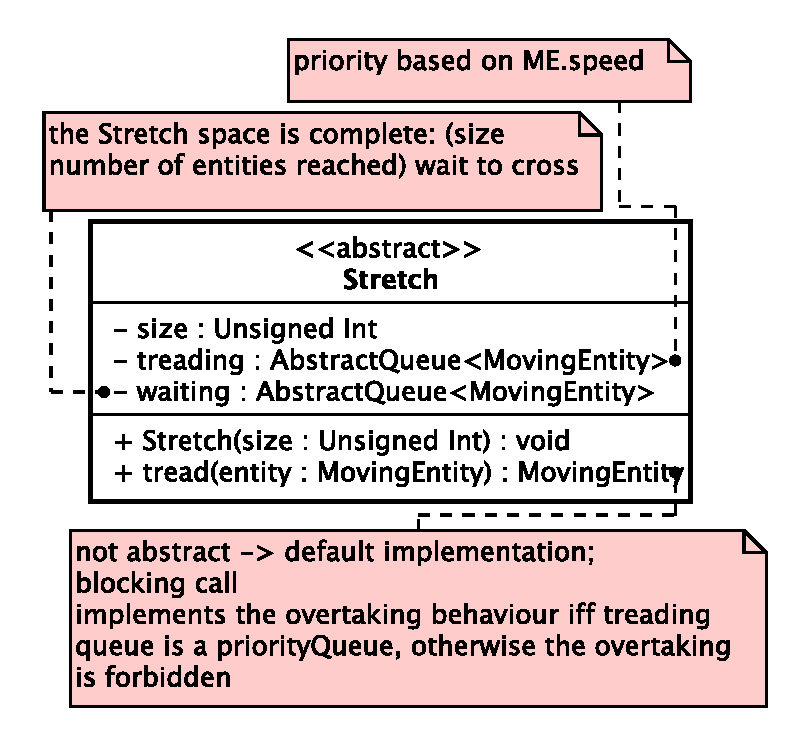
\includegraphics[scale=0.6,keepaspectratio]{images/solution/stretch.eps}
\caption{App::Reactive::Stretch}
\label{fig:sd-app-stretch}
\end{figure}
\FloatBarrier
\begin{itemize}
  \item \textbf{Description} \\
    It represents a stretch entity. It is a protected object.
  \item \textbf{Attribute}
  \begin{itemize}
    \item \texttt{- size: Unsigned Int} \\
The size of the stretch/treading queue.
    \item \texttt{- treading: AbstractQueue<MovingEntity>} \\
The queue of moving entities which are treading the stretch. If the concrete type
is PriorityQueue then the stretch allows the overtaking between the moving entities.
This is implemented through a priority queue ordered by decreasing speed.
    \item \texttt{- waiting: AbstractQueue<MovingEntity>} \\
The queue of moving entities which are waiting to tread the stretch. 
  \end{itemize}
  \item \textbf{Operation}
  \begin{itemize}
    \item \texttt{+ Stretch(size: Unsigned Int)} \\
Creates a stretch object with a specific size.
    \item \texttt{+ tread(entity: MovingEntity)} \\
Implements the stretch treading. The current speed of the moving entity
is calculated first, then the entity is placed in a treading queue which has a  
timeout. When this timeout expires, the queue is flushed and the entity can
proceed along their route.
  \end{itemize}
\end{itemize}
